\section{Dobór parametrów algorytmów PID i DMC}
Wykonano dwa skoki o różnej amplitudzie dla sygnału zadanego, 
na podstawie odpowiedzi obiektu dobrano nastawy regulatora PID metodą eksperymentalną. 
Ocena jakości regulacji na podstawie rysunków przebiegów sygnałów polega na ocenie jakościowej, 
analizowane są takie kryteria jak czas regulacji czy przeregulowanie. 
Na podstawie tych kryteriów oceny dobierane są nastawy regulatora PID.

Ocena jakości regulacji ilościowa polega na wyznaczaniu wskaźnika jakości regulacji, 
którym jest suma kwadratów uchybów. 

$$
E=\sum_{k=1}^{k_{konc}} \quad (y_{zad}(k)-y(k))^{2}
$$

Ocena jakości regulacji jakościowa jest metodą mniej dokładną od oceny ilościowej, 
nie występują tam obliczenia a jedynie analiza rysunków przebiegów. 
Podczas analizy rysunku osoba oceniająca jakość regulacji narażona jest na mało precyzyjne wnioski, 
gdyż należy wtedy zwracać uwagę na skalę rysunku i wiele innych parametrów. 
Ocena ilościowa nie bierze pod uwagę takich czynników jak np. oscylacje, 
jedynym kryterium jest suma kwadratów uchybów. 
Jeżeli do oceny jakości regulacji wymagane są inne kryteria niż podany wskaźnik 
jakości należy rozpatrzeć metodę oceny jakościowej. 

Wyniki doboru parametrów

Słaby PID Nastawy ?


  E = 612.3329

  E=559.2419


  E= 209.3488

  E=323.0685

  E=439.7029


\begin{figure}[H]
    \centering
    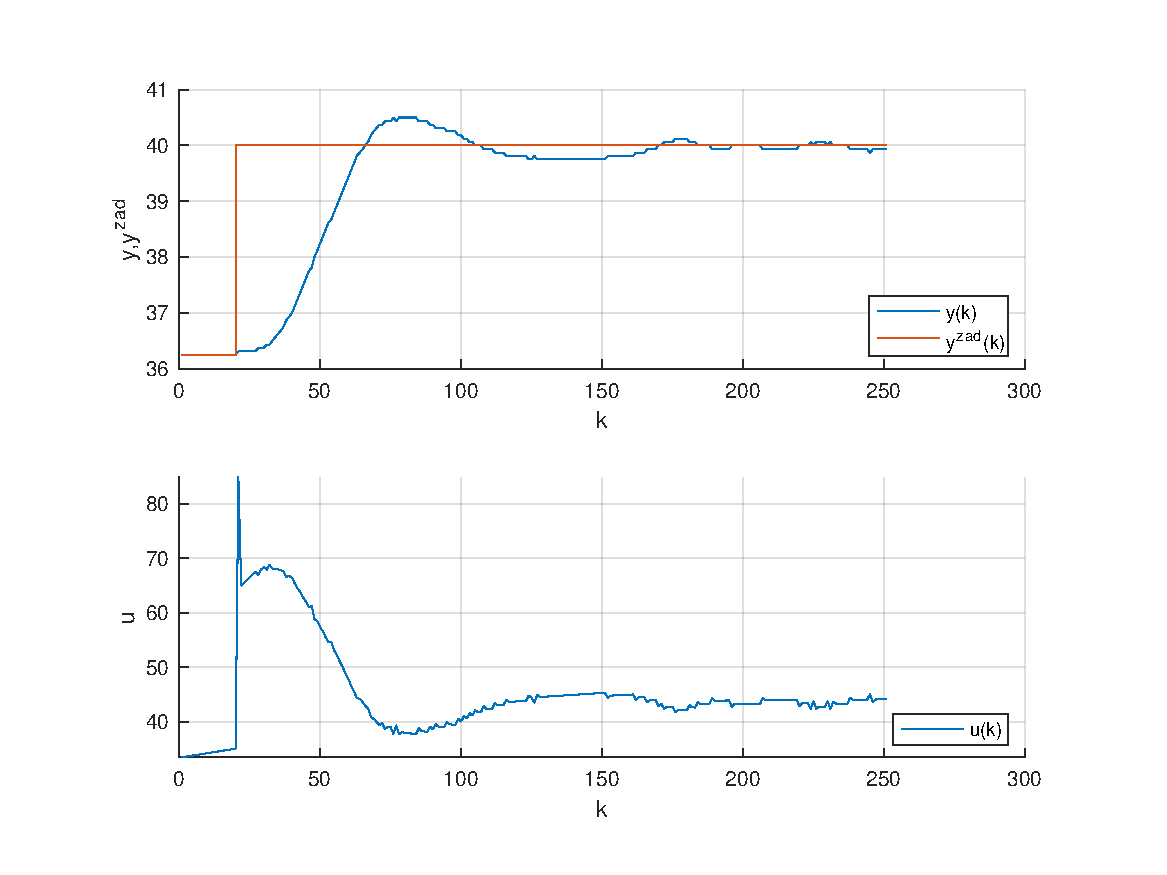
\includegraphics[scale=0.75]{../lab/zad_4/zad4pidd1.pdf}
    \caption{zad4pidd1}
\end{figure}

\begin{figure}[H]
    \centering
    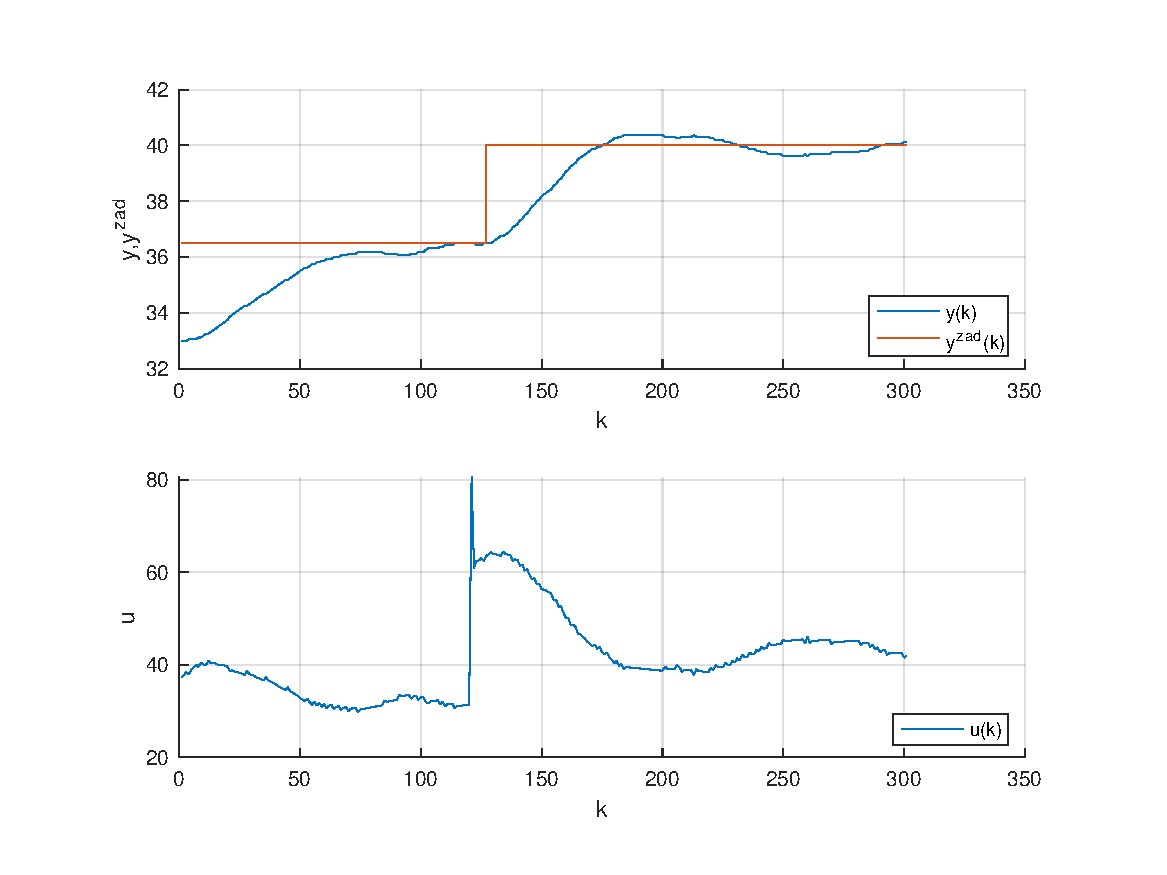
\includegraphics[scale=0.75]{../lab/zad_4/zad4pidd2.pdf}
    \caption{zad4pidd2}
\end{figure}

\begin{figure}[H]
    \centering
    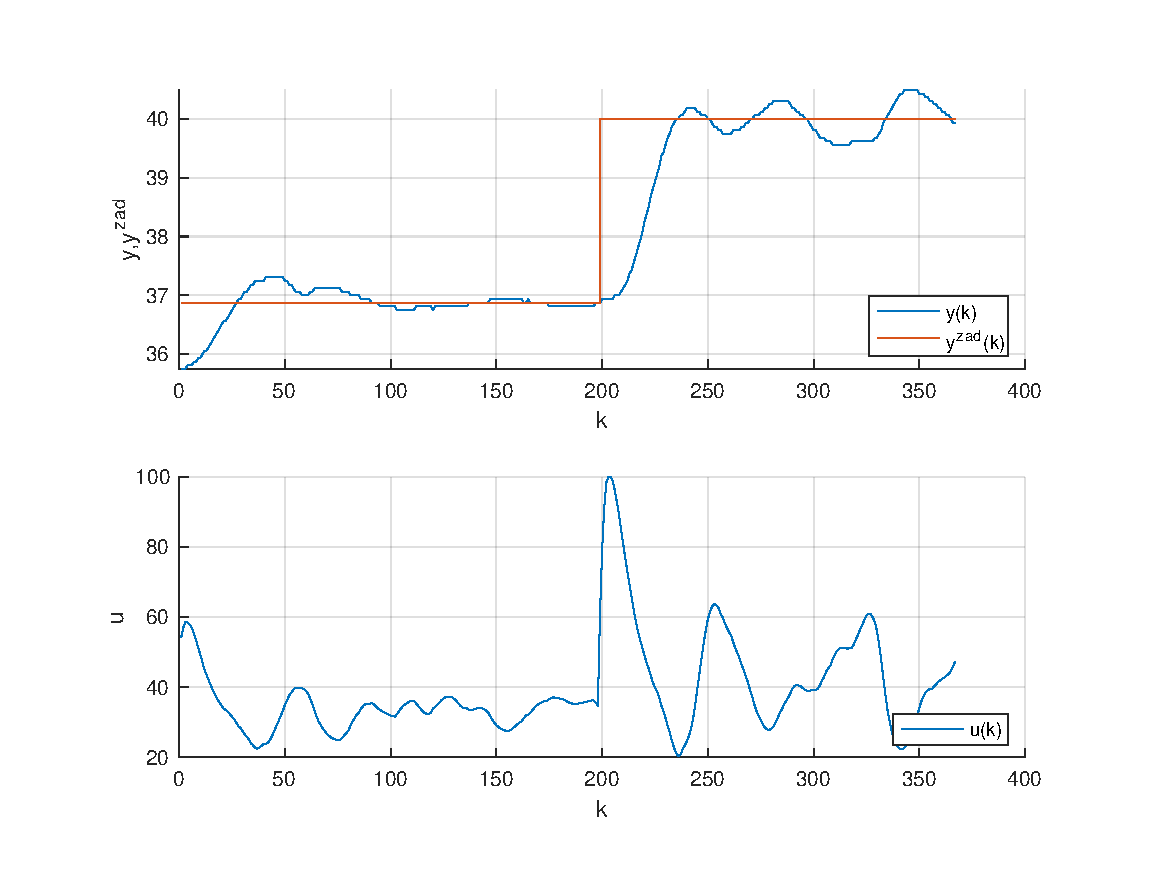
\includegraphics[scale=0.75]{../lab/zad_4/zad4dmc1.pdf}
    \caption{zad4dmc1}
\end{figure}

\begin{figure}[H]
    \centering
    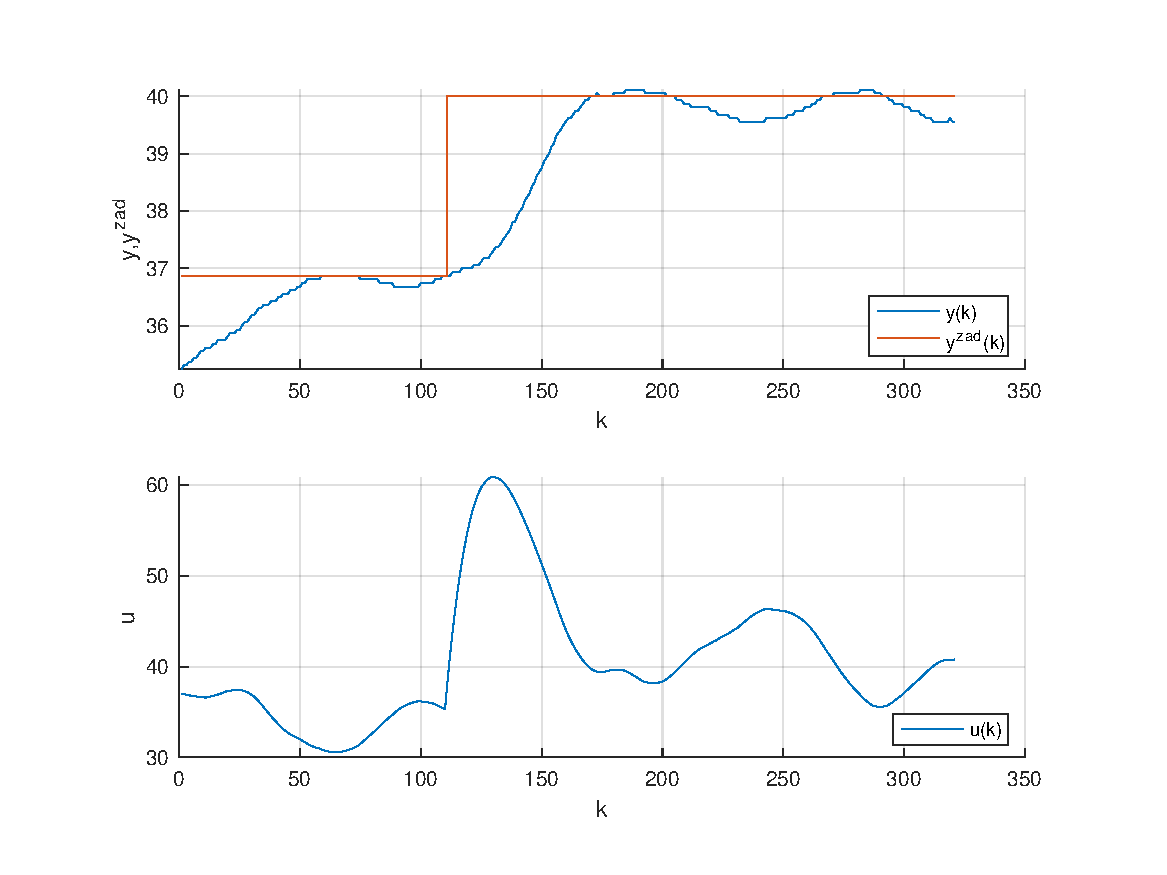
\includegraphics[scale=0.75]{../lab/zad_4/zad4dmc2.pdf}
    \caption{zad4dmc2}
\end{figure}

\begin{figure}[H]
    \centering
    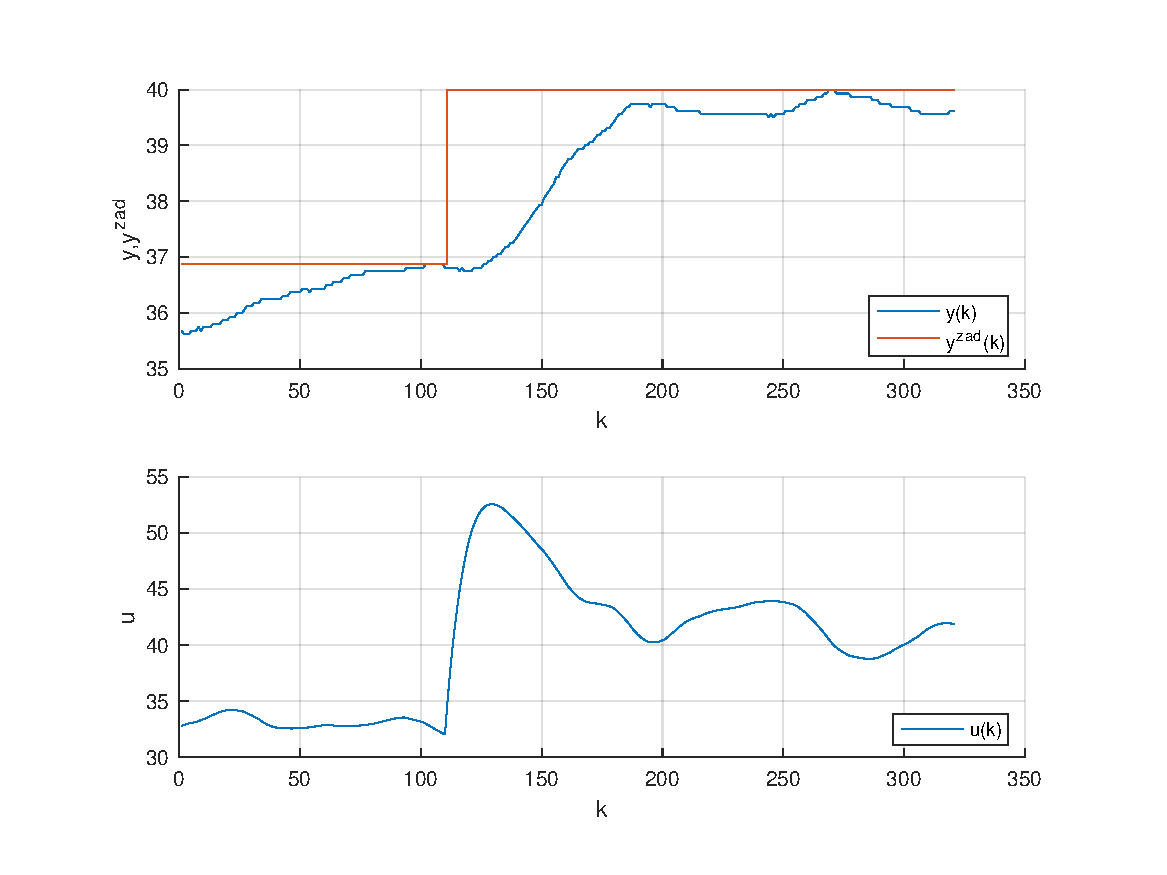
\includegraphics[scale=0.75]{../lab/zad_4/zad4dmc3.pdf}
    \caption{zad4dmc3}
\end{figure}
